\documentclass[landscape]{article}
\usepackage{amssymb,amsmath,amsthm,amsfonts}
\usepackage{multicol,multirow, bookmark}
\usepackage{calc}
\usepackage{ifthen}
\usepackage{graphicx}
\usepackage[landscape,a4paper,top=1cm,left=1cm,right=1cm,bottom=1cm]{geometry}
\usepackage{hyperref}

\pagestyle{empty}
\makeatletter
\renewcommand{\section}{\@startsection{section}{1}{0mm}%
                                {-0.5ex plus -.25ex minus -.1ex}%
                                {0.25ex plus .1ex}%
                                {\normalfont\normalsize\bfseries}}
\renewcommand{\subsection}{\@startsection{subsection}{2}{0mm}%
                                {-0.5ex plus -.25ex minus -.1ex}%
                                {0.25ex plus .1ex}%
                                {\normalfont\small\bfseries}}
\renewcommand{\subsubsection}{\@startsection{subsubsection}{3}{0mm}%
                                {-0.5ex plus -.25ex minus -.1ex}%
                                {0.5ex plus .1ex}%
                                {\normalfont\small\bfseries}}
\makeatother
\setcounter{secnumdepth}{0}
\setlength{\parindent}{0pt}
\setlength{\parskip}{0pt plus 0.5ex}

\title{Compilers}
\begin{document}


\tiny
\setlength{\linewidth}{\columnwidth}
\setlength{\hsize}{\columnwidth}

\begin{center}
     \Large{\textbf{Compilers}}
\end{center}

\begin{multicols*}{3}
\setlength{\premulticols}{1pt}
\setlength{\postmulticols}{1pt}
\setlength{\multicolsep}{1pt}
\setlength{\columnsep}{2pt}
\sloppy
\tolerance=1000
\emergencystretch=10pt


% DONE
\subsubsection{Key Definitions and Concepts}
A language L is LL(k) iff there is an LL(k) grammar G_L that accepts it, i.e.: L(G_L )= L.

An item is simply a grammar rule where we have inserted a • at some point in the right-hand part,
in order to makr the current progress of the CFSM
\section{Trivia}
Q:Give an advantage of hand-built scanners over automata-based scanners? 
A:They can go beyond regular languages

Q: How can we make sure the sequence 'true' is always deamed a contant and not a string?
A: Constants like 'true' should be recognized as a single token

Q: What is the longest match principle?
A: The principle states that when there is a choice between several possible matches during tokenization, the lexer should choose the longest possible match that forms a valid token.

Q: Argue that the exact of both type checking and reachability analysis are in fact undecidable.
A: The exact versions of both type checking and reachability analysis are undecidable because they would require solving the halting problem, which is proven to be undecidable. For type checking, determining the exact type of an expression in all possible cases would involve analyzing all potential program executions, which is equivalent to solving whether a program halts with certain inputs. Similarly, exact reachability analysis involves determining whether a specific program state can be reached, which also boils down to predicting the behavior of all possible executions, again leading to the halting problem. Since the halting problem is undecidable, both exact type checking and exact reachability analysis are also undecidable.


% TODO
% DONE

\subsection{Calculate First and Follow}
\subsubsection{First $^k(\alpha)$}
1. Initialization:
   For every terminal $a$, set $First^k(a) = {a}$ (since a terminal generates only itself).
   Initialize $First^k(A)$ to an empty set for every variable $A$.

2. Iterative Update:
   Repeat until no changes occur:
     For each variable $A$ with a production rule $A → X_1 X_2 ... X_n$:
     Compute $First^k(X_1)$, $First^k(X_2)$, ..., $First^k(X_n)$.
     Concatenate elements from $First^k(X_1)$, $First^k(X_2)$, ..., $First^k(X_n)$ and truncate the results to length $k$.
       Update $First^k(A)$ with these truncated elements if they are not already present.

3. Completion:
   The process stops when no $First^k$ sets are updated in an iteration, meaning all sets have stabilized.

\subsubsection{Follow $^k(\alpha)$}
1. Initialization:
   Initialize $Follow^k(X)$ to an empty set for each variable $X$.

2. Iterative Update:
   Repeat until no changes occur:
     For each rule $A → αBβ$:
       Compute $First^k(β)$ (where β is the part of the right-hand side following $B$).
       Add $First^k(β)$ elements to $Follow^k(B)$, completing them with $Follow^k(A)$ if needed to ensure they reach length $k$.
       Update $Follow^k(B)$ with these completed elements if they are not already present.

3. Completion:
   The process stops when no $Follow^k$ sets are updated in an iteration, meaning all sets have stabilized.


%\subsubsection{ItemFollows}

%TODO Done

\section{Canonical Finite State Machine Example}
Grammar:\\
$S \rightarrow A\$$\\
$A \rightarrow aCD$\\
$A \rightarrow ab$\\
$C \rightarrow c$\\
$D \rightarrow d$\\

CFSM:\\
% 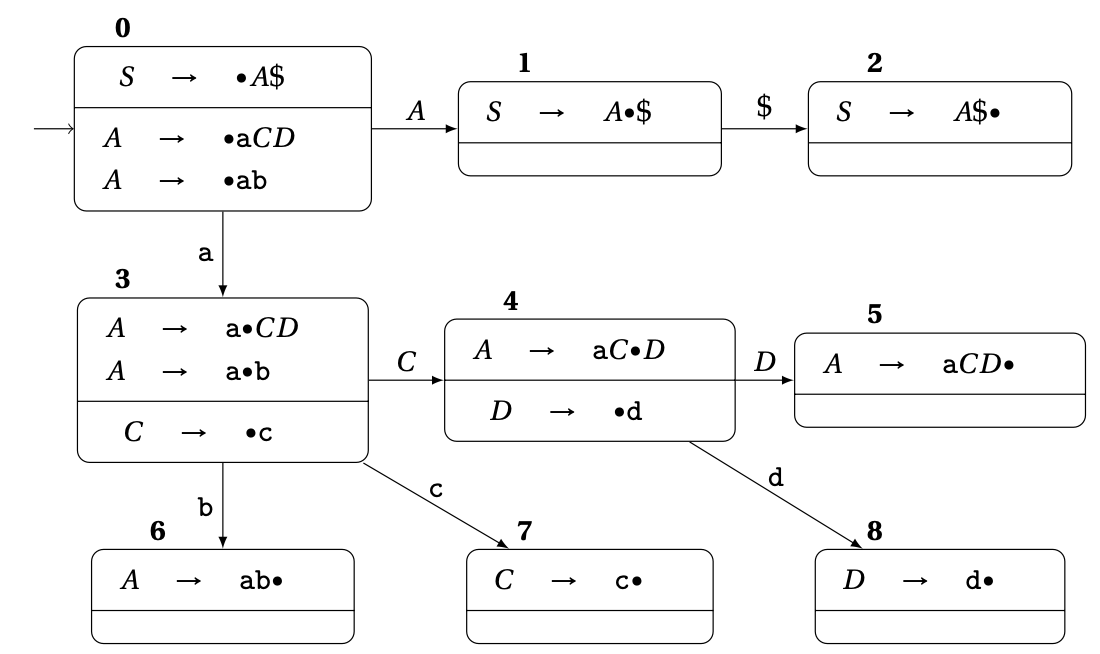
\includegraphics[height=5cm]{./images/Screenshot 2024-08-29 at 10.23.12.png}

The language of this grammar is LR(1).
\subsection{Grammars}

\subsubsection{LL(k)}

1. No Left Recursion: No non-terminal should be able to derive itself through a sequence of productions that starts with the same non-terminal. For example, a rule like $A \rightarrow A\alpha$ (where $\alpha$  is any sequence of terminals and/or non-terminals) would be left-recursive.

2. Left Factoring: For any non-terminal $A$ and productions $A \rightarrow \alpha \beta_1$ and $A \rightarrow \alpha \beta_2$ where $\alpha$ is a common prefix, the grammar should be refactored to remove the common prefix. The left-factored form would be:
   $A \rightarrow \alpha A'$\\
   $A' \rightarrow \beta_1 \mid \beta_2$

3. First/Follow Set Conditions: For each non-terminal $A$ and productions $A \rightarrow \alpha_1$ and $A \rightarrow \alpha_2$:
   The sets of terminals that can appear as the first token of the strings derived from $\alpha_1$ and $\alpha_2$ (i.e., the FIRST sets) must be disjoint.
   If $\alpha_i$ can derive the empty string $\epsilon$, then the FIRST set of $\alpha_i$ should not intersect with the FOLLOW set of $A$. The FOLLOW set of $A$ is the set of terminals that can appear immediately to the right of $A$ in some sentential form.



%SLR(k)

%LALR(k)

%LR(k)

\subsection{Languages}

\subsubsection{Regular langauges}
Regular languages are those that can be recognized by a finite automaton or expressed by a regular expression.

\subsubsection{Context-free languages}
Context-free languages are those that can be recognized by a pushdown automaton or expressed by a context-free grammar.
\subsection{Example Languages}
\textbf{LR(0) language that is not LL(1)}\\
    $L = \{a^n b^n | n \geq 0\}$

\textbf{LR(0) language that is not LL(k) for any k}\\
$L = \{a^n b^n c^m | n, m \geq 1\} $\

\textbf{LL(2) language that is not LL(1)}\\
$L = \{ a^n b c^n d \mid n \geq 1 \} \cup \{ a^n c b^n d \mid n \geq 1 \}$

\textbf{CFL that in not LR(1)}\\
    English language

\subsection{Example Grammars}
\textbf{LL(1) grammar that is not strongly LL(1)}\\
    $S \rightarrow A | B$\\
    $A \rightarrow aA | a$\\
    $B \rightarrow bB | b$

\textbf{LL(2) grammar that is not strongly LL(2)}\\
    $S \rightarrow A B$\\
    $A \rightarrow a A a | a$\\
    $B \rightarrow b B b | b$

\textbf{LALR(1) grammar that is not SLR(1)}\\
    $S \rightarrow A a$\\
    $A \rightarrow B b | C c$\\
    $B \rightarrow b$\\
    $C \rightarrow c$

\textbf{CFG that in not LR(1)}\\
    $S\rightarrow aB|aDc$\\
    $B\rightarrow bBc|c$\\
    $D\rightarrow bc|c$

\section{Parsing Grammar Proofs}

\subsection{LL(k) Proof}
A grammar is \textbf{LL(k)} if:
\begin{enumerate}
  \item No left recursion exists.
  \item For every non-terminal \(A\) with productions \(A \to \alpha \mid \beta\):
  \[
  \text{FIRST}_k(\alpha \cdot \text{FOLLOW}_k(A)) \cap \text{FIRST}_k(\beta \cdot \text{FOLLOW}_k(A)) = \emptyset
  \]
  (If \(\alpha\)/\(\beta\) can derive \(\epsilon\), include \(\text{FOLLOW}_k(A)\).)
\end{enumerate}

\subsection{SLR(k) Proof}
A grammar is \textbf{SLR(k)} if:
\begin{enumerate}
  \item Construct SLR(1) states (LR(0) items + \text{FOLLOW} for reduce actions).
  \item No \textit{shift-reduce} or \textit{reduce-reduce} conflicts in the parsing table.
  \item Conflicts tested using \text{FOLLOW} sets (not lookaheads).
\end{enumerate}

\subsection{LR(k) Proof}
A grammar is \textbf{LR(k)} if:
\begin{enumerate}
  \item Construct canonical LR(k) states (with full lookaheads).
  \item No conflicts in the parsing table (even with precise lookaheads).
\end{enumerate}

\subsection{LALR(k) Proof}
A grammar is \textbf{LALR(k)} if:
\begin{enumerate}
  \item Merge LR(1) states with identical \textit{cores} (same productions, different lookaheads).
  \item Ensure no conflicts arise after merging (common in practice but weaker than LR).
\end{enumerate}

\subsubsection*{Hierarchy}
\[
\text{SLR} \subset \text{LALR} \subset \text{LR}, \quad \text{LL} \subset \text{CFG (non-overlapping)}
\]


\textbf{Key Notes}:
- For \textbf{LL(k)}: Compute \(\text{FIRST}_k\) and \(\text{FOLLOW}_k\) rigorously.
- For \textbf{SLR}: Conflicts = overlap between shift terminals and \(\text{FOLLOW}\) of reduced non-terminal.
- \textbf{LALR} merges LR(1) states; conflicts here imply not LALR but might still be LR.
- \textbf{Left recursion} invalidates LL(k); \textbf{ambiguity} invalidates all.


\end{multicols*}

\end{document}
